\documentclass[9pt,a4paper]{article}
\usepackage[utf8]{inputenc}       
\usepackage[english,russian]{babel}
\usepackage{PTSerif}                
\usepackage[pdftex]{graphicx}        
\usepackage{layout}                   
\usepackage{fancyhdr}                  
\usepackage{fullpage}                   
\usepackage{array}                       
\usepackage{longtable}                    
\usepackage{listings}
\usepackage{footnote}                       
                                             
\setlength\voffset{-1in}                      
\setlength\hoffset{-1in}                       
\setlength\topmargin{1cm}                       
\setlength\oddsidemargin{2cm}                    
\setlength\textheight{25.7cm}                     
\setlength\textwidth{17.001cm}                     
\setlength{\topskip}{1.3cm}                         
\setlength\headheight{0cm}                           
\setlength\headsep{0cm}                               
                                                       
\pagestyle{fancyplain}                                  
\fancyhf{}                                               
\cfoot{\small\em \textcopyright \hspace{0.1em} ARCСN 2013}
\rfoot{\small \thepage}

\renewcommand{\labelitemii}{$\circ$}
                                      
\title{Руководство по HCProbe}
\author{Александр Вершилов, Кирилл Заборский}

\begin{document}
\maketitle
\begin{figure}[!h]
   \centering 
   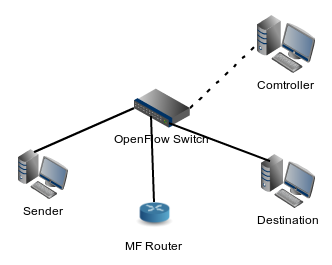
\includegraphics[width=0.3\columnwidth]{images/testcfg2.png}
\end{figure}                                                        

\tableofcontents

\pagebreak

\section{Общее описание}

\textbf{HCProbe}~--- средство тестирования OpenFlow контроллеров, которое
содержит реализацию библиотеки для работы с протоколом OpenFlow на языке
Haskell, предоставляет эталонную реализацию программного OpenFlow свича и язык
для создания новых свичей.

\subsection{Перечень терминов}

\begin{description}
  \item[OpenFlow] протокол управления процессом обработки данных, передающихся
    по сети передачи данных маршрутизаторами и коммутаторами, реализующий
    технологию программно-конфигурируемой сети (SDN).
  \item[EDSL] встроенный предметно-ориентированный язык
\end{description}

\pagebreak

\section{Подсистемы}

В проекте HCProbe можно выделить следующие подсистемы:

\begin{description}
    \item[библиотека OpenFlow] -- реализация OpenFlow протокола;
    \item[OpenFlow/Ethernet] -- реализация генерации Ethernet-кадров, содержащих
      пакеты протоколово более высоких уровней;
    \item[HCProbe] -- реализация эталонного программного свича OpenFlow, который
      осуществляет отправку сообщений PacketIn;
    \item[HCProbe/EDSL] -- предметно-ориентированный язык для создания
      контроллеров;
    \item[тесты] -- тесты создания и разбора пакетов;
    \item[примеры] -- примеры тестов для OpenFlow-контроллеров, разработанные с
      использованием предметно-ориентированного языка.
\end{description}


\subsection{Библиотека OpenFlow}

Библиотека OpenFlow представляет собой поддержку протокола OpenFlow,
описываемого стандартом OpenFlow Switch Specification, Version 1.0.0
\footnote{http://www.openflow.org/documents/openflow-spec-v1.0.0.pdf} для
\texttt{Haskell}. Основные модули подсистемы:

\begin{description}
    \item[Network.Openflow.Types] -- реализация структур данных, соответствующая
      структурам данных OpenFlow протокола:
        \begin{itemize}
            \item инстансы \textbf{Binary.Read} для разбора структур;
            \item инстансы \textbf{Enum} для всех перечислений.
        \end{itemize}
    \item[Network.Openflow.Misc] -- дополнительные функции, использующиеся в
      библиотеке:
        \begin{itemize}
            \item функции подсчета CRC;
            \item функции сериализации специальных типов данных;
            \item функции работы с IP и MAC адресами.
        \end{itemize}
    \item[Network.Openflow.Messages] -- функции сериализации и разбора сообщений
      OpenFlow.
\end{description}

\emph{Реализация протокола не является полной, так реализованы не все структуры
  из спецификации, однако, расширение поддерживаемого протокола может
  выполняться по аналогии с уже написанным кодом.}

\subsection{OpenFlow/Ethernet}

Данная подсистема предоставляет интерфейс для создания пакетов протоколов
сетевого стека (Ethernet, IPv4, ARP, TCP). Таким образом, можно создавать
специальные тестовые пакеты для инкапсуляции в сообщения PacketIn.

Основные модули:

\begin{description}
  \item[Network.Openflow.Ethernet] -- реэкспортирование всех модулей, достаточно
    использовать только его
  \item[Network.Openflow.ARP]      -- ARP пакет
  \item[Network.Openflow.Frame]    -- Ethernet кадр
  \item[Network.Openflow.IPv4]     -- IPv4 пакет
  \item[Network.Openflow.TCP]      -- TCP пакет
  \item[Network.Openflow.Types]    -- внутренние типы данных
\end{description}

\subsection{HCProbe}

HCProbe является исполняемым файлом, реализующим набор программных свичей,
которые могут быть взяты за эталонную реализацию программного OpenFlow свича.

Программа \texttt{hcprobe} создает указанное количество виртуальных свичей,
которые соединяются c контроллером, после чего начинают отправлять контроллеру
сообщения PacketIn.  Данные сообщения PacketIn содержат Ethernet-кадр, в
заголовке которого указываются MAC-адреса, выбранные из множества MAC-адресов
хостов, относящихся к тому или иному порту свича.  Ethernet-кадр, в свою
очередь, содержит IP-пакет с сегментом TCP.

В ходе выполнения программы выводится статистика, содержащая количество
отправленных и полученных сообщений, среднее время обработки контроллером одного
сообщения, а также количество потерянных сообщений и количество закрытых
соединений.

\subsection{EDSL}

Предметно-ориентированный язык HCProbe предназначен для описания свичей
OpenFlow, создания программ, описывающих работу отдельных свичей и их
комбинаций, а также для регистрации и сбора статистики по обмену сообщениями
между свичами и контроллером OpenFlow.

\subsubsection{Структура программы}

Типовая программа, написанная с использованием предметно-ориентированного языка
HCProbe, включает, как минимум, 2 части:

\begin{itemize}
  \item Создание свича и задание его конфигурации;
  \item Запуск свича в соответствии с требуемой программой.
\end{itemize}

Кроме этого в большинстве случаев требуется 3-й шаг, на котором программа
дожидается завершения работы свичей (одного или нескольких в зависимости от
задачи) и формирует итоговую сводку статистики по запуску.

\subsubsection{Создание свича}

Свич создается одной из команд \lstinline!switch! или \lstinline!switchOn!. В
первом случае в качестве образца будет использован свич с конфигурацией по
умолчанию, а во-втором~--- свич, переданный как параметр. Таким образом, командой
\lstinline!switchOn! можно получить копию свича, созданного ранее.

Для того, чтобы диапазоны MAC-адресов свичей не пересекались, используется окружение
\lstinline!config!, в котором они и создаются:

\begin{lstlisting}
    sw <- config $ switch <switchIP> $ do ..
\end{lstlisting}%$

\subsubsection{Настройка возможностей свича}

Настройки свича проводятся в окружении \lstinline!features!, в котором можно
задать параметры свича.

\begin{lstlisting}
    switch <switchIP> $ do
      features $ do
        ..
\end{lstlisting}

К настройкам относятся, например, порты, добавляемые командой
\lstinline!addPort!.

Команда \lstinline!addMACs! добавляет список MAC-адресов к свичу, при этом они
разделяются поровну между портами этого свича.

\emph{Как было указано выше, для предотвращения пересечения диапазонов
  MAC адресов разных свичей иcпользуется окружение \lstinline!config!,
  таким образом, если при задании списка MAC адресов какого-либо свича
  будет выявлено пересечение с другими свичами, то вместо
  пересекающихся адресов этому свичу будут присвоены MAC адреса из ещё
  не занятых}

\lstinline!clearMACs! удаляет все MAC-адреса, добавленные к свичу.


\subsubsection{Запуск свича}

Свич может быть запущен в 2 вариантах:

\begin{itemize}
  \item если для задачи подходит стандартная реализация логики свича, то
    запускать его следует при помощи функции \lstinline!runSwitch!;
  \item чаще требуется задание какой-то конкретной логики поведения свича,
    которая может быть задана при выполнении функции \lstinline!withSwitch!.
\end{itemize}


\subsubsection{Выполнение программы}
После запуска свича (при помощи \lstinline!withSwitch!) он начианет выполнять
переданную ему программу. Данный блок является обычным блоком кода на haskell,
который может взаимодействовать со свичем, используя созданные для этого
команды, среди которых есть следующие:

\begin{description}
  \item[hangOn] -- ожидать вечно, может быть полезно в случае, если нужно
    тестировать свич.

  \item[waitForType] -- ожидание определенного типа сообщения: выполнение
    прогаммы будет приостановлено то тех пор, пока не придет сообщение
    указанного типа. Возвращает полученное сообщение.

  \item[waitForBID] -- ожидание сообщения с указанным значением
    \lstinline!buffer id!.  Возвращшает полученное сообщение.

\end{description}

Для генерации сообщений желательно, чтобы используемые номера транзакций и
буферов не пересекались, для этого служат команды \lstinline!nextBID! и
\lstinline!nextTID!.

Для отправки сообщений могут быть использованы следующие команды:

\begin{description}

  \item[send] -- отправка произвольного сообщения OpenFlow контроллеру;

  \item[sendOFPacketIn] -- отправка сообщения типа \lstinline!OFPT_PACKET_IN!;

  \item[sendARPGreeting] -- отправка сообщения типа \lstinline!OFPT_PACKET_IN!
    с ответом ARP внутри (может использоваться для того, чтобы сообщить
    контроллеру все доступные свичам MAC-адреса до начала тестирования);

  \item[statsSend/statsSendOFPacketIn] -- варианты \lstinline!send! и
    \lstinline!sendOFPacketIn! со сбором статистики при отсылке пакетов.

\end{description}

\subsubsection{Сбор статистики}

Текущая реализация поддерживает сбор следующих параметров статистики:

\begin{itemize}
  \item число отосланных сообщений;
  \item число сообщений с ответами от контроллера;
  \item число сообщений без ответов от контроллера (сообщения в очереди
    становятся потерянными, если очередь переполняется);
  \item времена ответов от сервера (вычисляются как разница времён отправки
    сообщения и получения ответа на него).
\end{itemize}

Использование статистики подразумевает следующие шаги:

\begin{itemize}
  \item вызов \lstinline!initPacketStats! для создания cущности
    \lstinline!StatsEntity!, в которой будут храниться данные статистики;
  \item регистрация обработчика статистики для свича при помощи
    \lstinline!setSilentStatsHandler! или \lstinline!setStatsHandler stEnt ...!.
    Первый вариант не выводит никакой информации в консоль или файл.  Второй
    вариант позволяет задать произвольное действие при получении ответа на
    сообщение, например, выводить в консоль или в файл время обработки
    сообщения контроллером (round trip time);
  \item отсылка сообщения контроллеру при помощи команд \lstinline!statsSend!
    или \lstinline!statsSendOFPacketIn!;
  \item получение сводной статистики по контроллерам при помощи команды
    \lstinline!assembleStats!.
\end{itemize}

\subsubsection{Изменение ответов контроллеру по умолчанию}

Для того, чтобы изменить поведение свича при получении определенных типов
сообщений от контроллера (например, для проверки реакции контроллера на
ошибочное поведение свича, потерю пакетов и т.п.)  можно использовать команду
\lstinline!setUserHandler!, которая позволяет задать необходимую реакцию.

\emph{В текущей реализации статистика работает также через
  \lstinline!setUserHandler!, поэтому одновременно оба эти механизма (получение
  статистики и формирование своих ответов контроллеру) пока использовать не
  рекомендуется.}

\section{Приложения}

\subsection{Параллельная работа нескольких программных свичей}

Для параллельного запуска нескольких свичей и контроля за временем исполнения
используется библиотека asyc\footnote{http://hackage.haskell.org/package/async}

Самым простым приёмом может быть ограничение времени выполнения свича:

\begin{lstlisting}
import Control.Concurrent (threadDelay)
import Control.Concurrent.Async (race_)

...
race_ action1 (threadDelay 1000000)
\end{lstlisting}

Здесь подразумевается, что action1 содержит запуск нужного свича, таким образом,
выполнение этой строки завершится или по завершении программы свича (если она
отличается от программы по умолчанию и конечна), или по истечении одной секунды.

Если же запускается одновременно несколько свичей, то типовым решением будет
запуск каждого из них в отдельном потоке (при помощи \lstinline!async!) и
ожидание их завершения (или истечения интервала времени, если это необходимо).

Схематически это будет выглядеть следующим образом:

\begin{lstlisting}
  a1 <- async $ withSwitch sw1 ...
  ...
  aN <- async $ withSwitch swN ...
  mapM_ waitCatch [a1,....,aN]
\end{lstlisting}

Если выполнение программы стоит приостановить при появлении ошибки в любом из
свичей, то \lstinline!waitCatch! следует заменить на \lstinline!wait!.

Вместо \lstinline!withSwitch! может стоять \lstinline!runSwitch!
в зависимости от задачи.

\subsection{Примеры программ}

\subsubsection{Простейший свич}

Это один из простейших примеров, в котором задаётся 2 свича, выводится в консоль
конфигурация второго и запускается первый с программой по умолчанию с
ограничением работы в 3 секунды.

\begin{lstlisting}
{-# LANGUAGE OverloadedStrings #-}
module Main
  where

import Control.Concurrent (threadDelay)
import Control.Concurrent.Async (race_) -- EDSL for asynchronous actions
import Data.Bits                        -- for IP creation
import HCProbe.EDSL

main = do 
    let ip = 15 .|. (0x10 `shiftL` 24)
    (sw1,sw2) <- config $ do
      sw1 <- switch ip $ do
            features $ do
                {- replicateM 48 $ --uncomment to create 48 ports -}
                addPort [] [] [OFPPF_1GB_FD, OFPPF_COPPER] def
                addPort [] [] [OFPPF_1GB_FD, OFPPF_COPPER] def
            addMACs [1..450]
      sw2 <- switchOn sw1 $ do
                clearMACs 
                addMACs [400..500]
      return (sw1,sw2)
    print sw2
    race_ (runSwitch sw1 "localhost" 6633) (threadDelay 3000000)
\end{lstlisting}

\end{document}
